%!TEX root = ../../main.tex

\chapter{Datenmodell und Mengengerüst}
In Abbildung \ref{fib:Datenmodell} sind die von der Software veralteten Daten und ihre Beziehungen untereinander modelliert.

\begin{figure}[h]
\centering
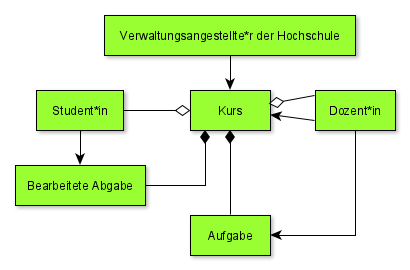
\includegraphics[height=.5\textwidth]{Datenmodell.png}
\caption{Datenmodell für die Anwendung eCourse}
\label{fib:Datenmodell}
\end{figure}

In Tabelle \ref{tab:Mengengerüst} finden sich die Datenmengen, mit der die Software arbeiten wird.

\begin{table}
\centering
	\begin{tabularx}{\textwidth}[H]{|X|X|}
		\hline
		Verwaltungsangestellte*r der Hochschule & Anzahl der Verwaltungsangestellten der Hochschule, meist im Bereich von 1 bis 100  \\
		\hline 
		Student*in & Anzahl der Studierenden der Hochschule, meist im Bereich zwischen 1000 und 10000 \\
		\hline
		Dozent*in & Anzahl der Dozierenden der Hochschule, meist im Bereich zwischen 100 und 1000\\
		\hline
		Kurs & Anzahl der Kurse, zu beachten ist, dass Kurse für eine bestimmte Zeit archiviert werden müssen, meist im Bereich zwischen 10.000 und 100.000 \\
		\hline
		Aufgabe & Pro Kurs meist im Bereich zwischen 1 und 10 \\
		\hline
		Bearbeitete Abgaben & Pro Aufgabe im Bereich der Studierenden pro Kurs \\
		\hline
	\end{tabularx}
\caption{Mengengerüst für die Anwendung eCourse}
\label{tab:Mengengerüst}
\end{table}